%----------------------------------------------------------------------------------------
%	PACKAGES AND THEMES
%----------------------------------------------------------------------------------------
\documentclass[aspectratio=169,xcolor=dvipsnames,8pt]{beamer}
\usetheme{Simple}

\usepackage{hyperref}
\usepackage{graphicx} % Allows including images
\usepackage{booktabs} % Allows the use of \toprule, \midrule and \bottomrule in tables
\usepackage{tikz}
\newcommand{\beq}{\begin{equation}}
\newcommand{\eeq}{\end{equation}}
\newcommand{\bes}{\begin{split}}
\newcommand{\ees}{\end{split}}
\newcommand{\BB}{\textbf{B}}
\newcommand{\jj}{\textbf{j}}
\newcommand{\x}{\times}
\newcommand{\ii}{\iota}
\newcommand{\iotaa}{\bar{\iota}}
\newcommand{\dd}{\partial}
\graphicspath{{./Figures/}}  

\setbeamersize{text margin left=14mm,text margin right=14mm}


%----------------------------------------------------------------------------------------
%	TITLE PAGE
%----------------------------------------------------------------------------------------

% The title
\title[Summary]{Numerical study of the effect of secondary electron emission on the dynamics of electron clouds in gyrotron guns}

\author[S.Guinchard] {S. ~Guinchard$^{1}$, G. ~Le Bars$^{2}$}
\institute[SPH] % Your institution may be shorthand to save space
{
    % Your institution for the title page
    $^1$ Ecole Polytechnique Fédérale de Lausanne (EPFL), Physics Section (SPH), CH-1015 Lausanne, Switzerland\\
    $^2$ Ecole Polytechnique Fédérale de Lausanne (EPFL), Swiss Plasma Center (SPC), CH-1015 Lausanne, Switzerland\\
    \vspace{1cm}
}
\date{\today} % Date, can be changed to a custom date

% Backgorund
\usebackgroundtemplate%
{%
    
\includegraphics[width=\paperwidth,height=\paperheight]{Figures/Backgroup-4.png}%
}



%----------------------------------------------------------------------------------------
%	PRESENTATION SLIDES
%----------------------------------------------------------------------------------------

\begin{document}

\begin{frame}
    % Print the title page as the first slide
    \titlepage
\end{frame}

% %------------------------------------------------
%%%%%%%%%%%%%%%%%%%%%%

\begin{frame}{Problem description}

\begin{itemize}


\item{Code espic2D does not take account (yet) for secondary electron emissions, induced by ions collected at the electrodes. Let us denote these ion-induced electron emissions by IIEE from now on.
}
\item{Goal: Implement a module to add those IIEE to espic2D 
}
\end{itemize}
\end{frame}

%-------------------------------------------------
%%%%%%%%%%%%%%%%%%%%%%%

\begin{frame}{Model to be used}

\begin{itemize}


\item{We seek an expression for the \textbf{electron yield} $\gamma$ 
}
\item{It is expected that $\gamma$ depends on the \textbf{incident particle energy}, the target density i.e a \textbf{material parameter} including cross sections for particle interactions, as well as \textbf{transport phenomena} occurring for produced electrons.
}

\item{ Semi-empirical model: \textbf{Schou} (1988) [Hassel92]
\beq
\gamma = \Lambda\cdot \beta \cdot \frac{dE}{dx}\Bigg|_{e}\label{Schou_eq}
\eeq
}

\item{In the above Eq.(\ref{Schou_eq}), $\Lambda$ includes the cross sections for collisions with energy deposition, $\beta$ accounts for energy transport by recoil electrons, and $dE/dx$ corresponds to the energy deposed in the solid by the ion colliding with electrons (subscript $e$).
}

\end{itemize}

\end{frame}

%-------------------------------------------------
%%%%%%%%%%%%%%%%%%%%%%

 \begin{frame}{Empirical values for model parameters}
     \begin{columns}[c] % The "c" option specifies centered vertical alignment while the "t" option is used for top vertical alignment

         \column{.5\textwidth} % Left column and width
	\begin{itemize}


		\item{Research of tabulated values (semi-empirical model) for the physical parameters:\\
			\begin{itemize}
		
				\item{$dE/dx$ from [Janni]}
				\item{$\beta$ and $\Lambda = \Lambda_{exp}$ from [Hassel92]}
				\end{itemize}}
				
						
	\end{itemize}

         \column{.5\textwidth} % Right column and width
		\begin{figure}[h!]
		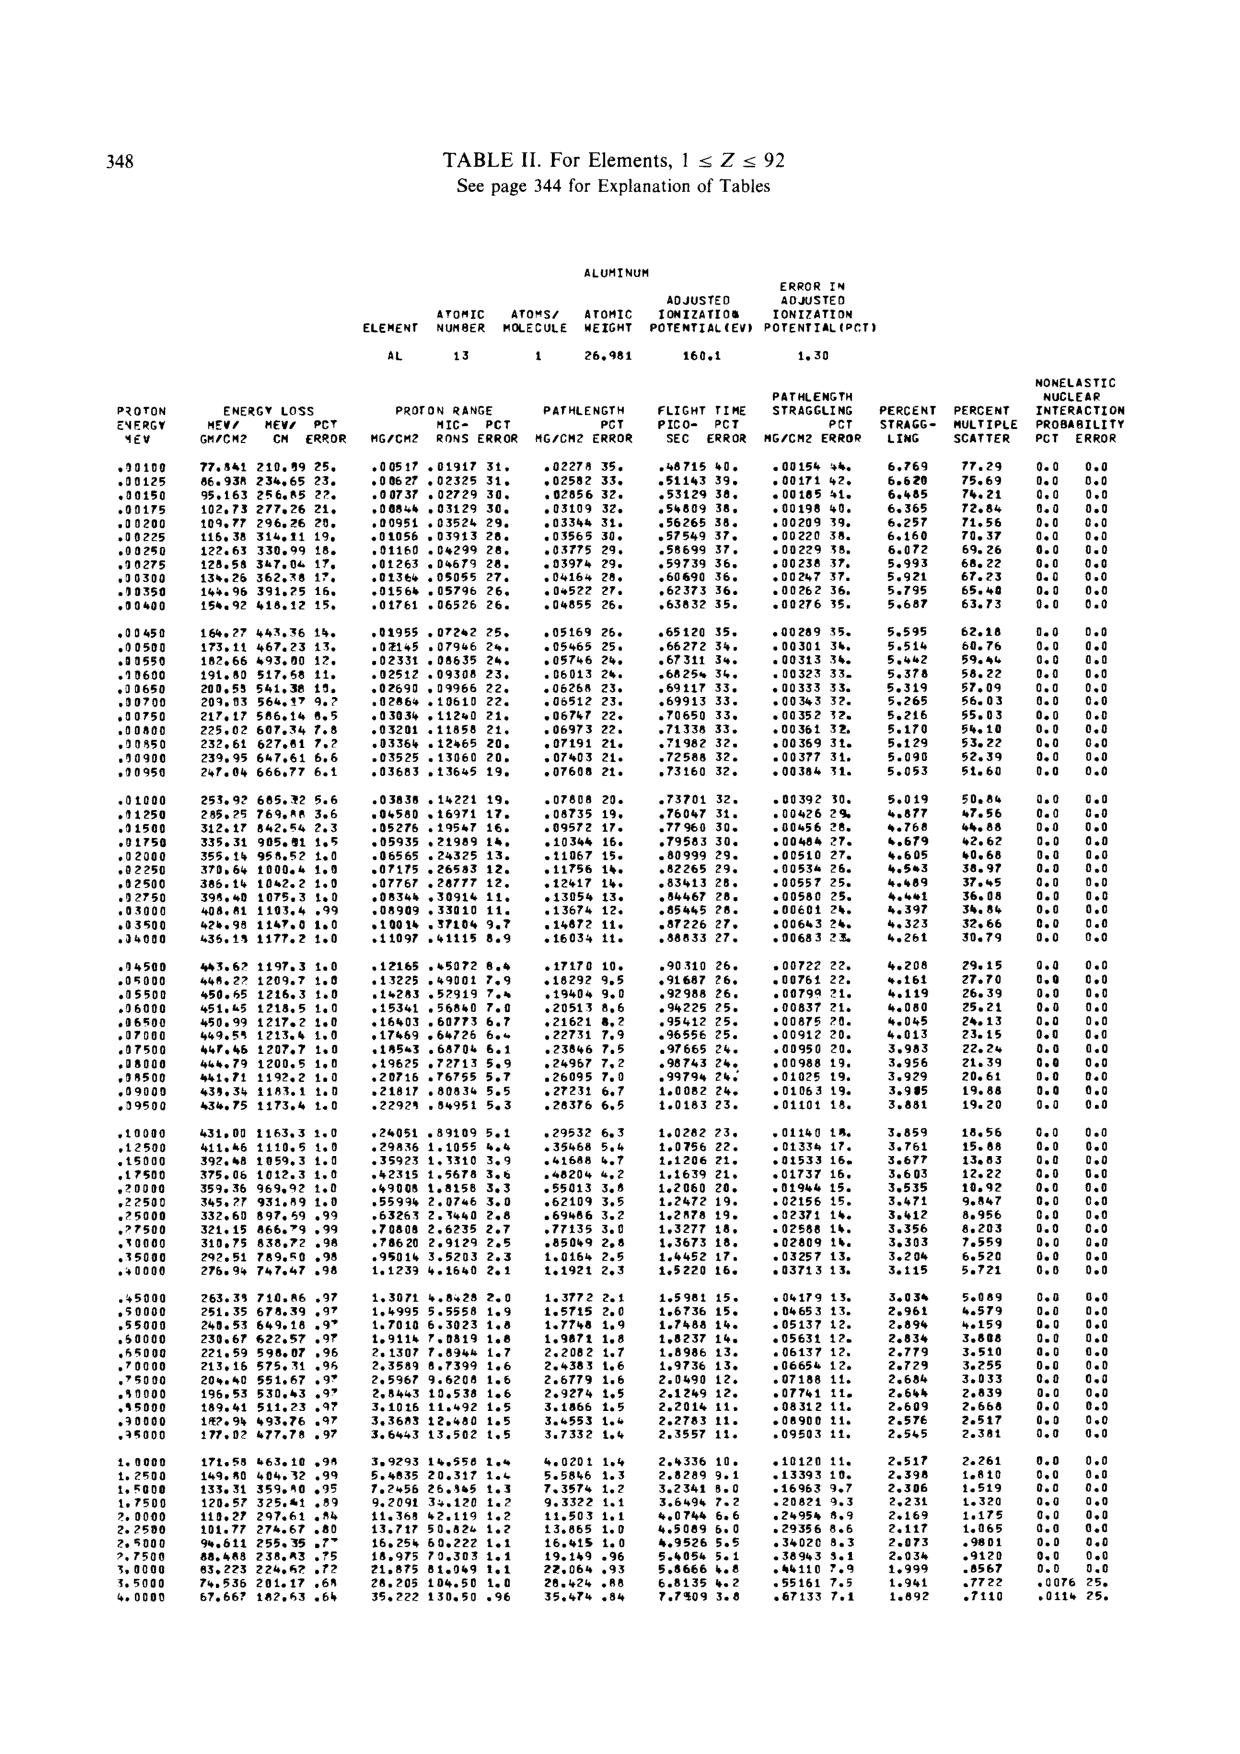
\includegraphics[width=0.7 \textwidth]{Al-table.pdf}
		\caption{\label{img1} Energy loss values from [Janni82]}
		\end{figure}
     \end{columns}
\end{frame}
% %------------------------------------------------
%%%%%%%%%%%%%%%%%%%%%

 \begin{frame}{Appropriate fit for the data}
     \begin{columns}[c] % The "c" option specifies centered vertical alignment while the "t" option is used for top vertical alignment

         \column{.5\textwidth} % Left column and width
	\begin{itemize}


		\item{In order to implement the energy loss of deposed ions, we need to find the appropriate fit:\\
		To do so, one has to determine the \textbf{energy distribution of ions collected at the electrode}, and match it with the energy loss curve.
		}
		\item{In Fig.(\ref{fig2}), the energy loss of protons in Aluminum has been plotted on the expected energy range of $20$ keV to $1$ GeV (see red curve).\\
		E.g if the protons are mainly distributed in parabolic region (green) $\rightarrow$ quadratic fit\\
		Else a linear fit may be more appropriate.
		}
				
						
	\end{itemize}

         \column{.5\textwidth} % Right column and width
		\begin{figure}[h!]
		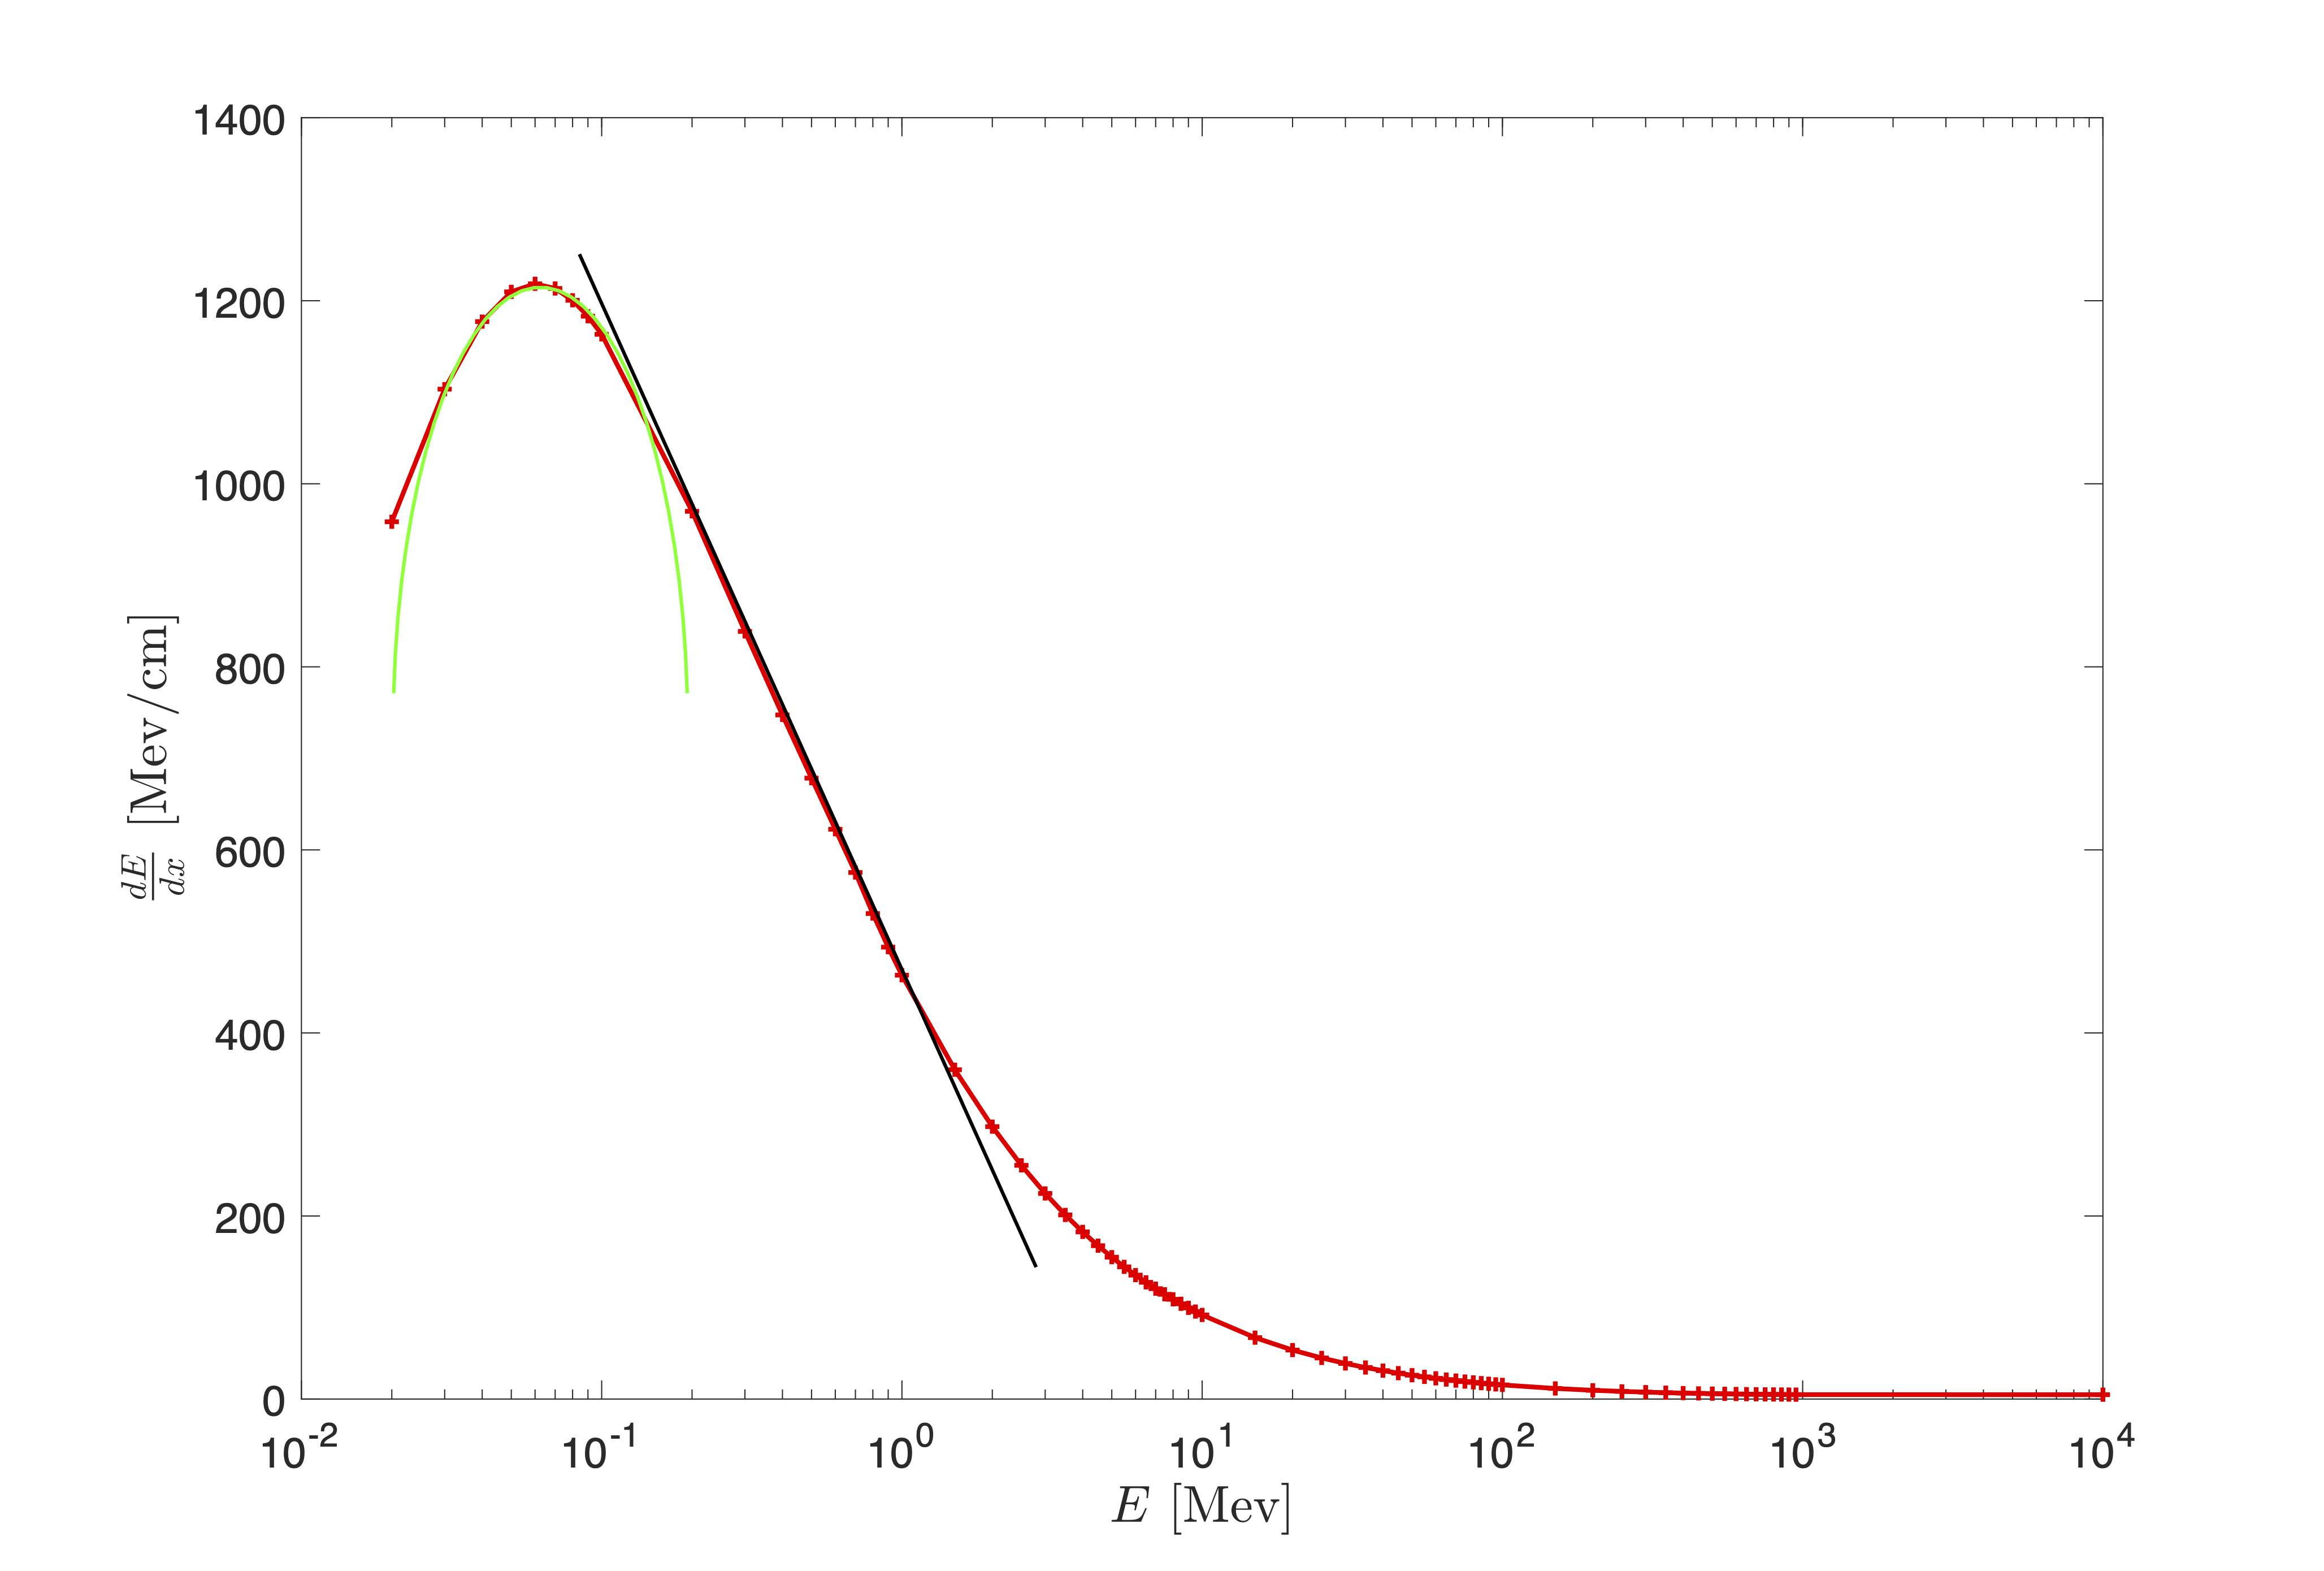
\includegraphics[width=1 \textwidth]{fit.png}
		\caption{\label{fig2} Energy loss for protons in aluminum (red) - possible fits for the data in interesting regions (green - black)}
		\end{figure}
     \end{columns}
\end{frame}
% %------------------------------------------------
%%%%%%%%%%%%%%%%%%%%

\begin{frame}{Initial configuration}
     \begin{columns}[c] % The "c" option specifies centered vertical alignment while the "t" option is used for top vertical alignment

         \column{.5\textwidth} % Left column and width
	\begin{itemize}


		\item{Initial configuration: generation of ions with maxwelian velocity profile}
		\item{Cylindrical symmetry and ions generated at different $r = R_0$}
		\item{Potential bias of $~20kV$ - radial $\mathbf{E}$}
				
						
	\end{itemize}

         \column{.5\textwidth} % Right column and width
		\begin{figure}[h!]
		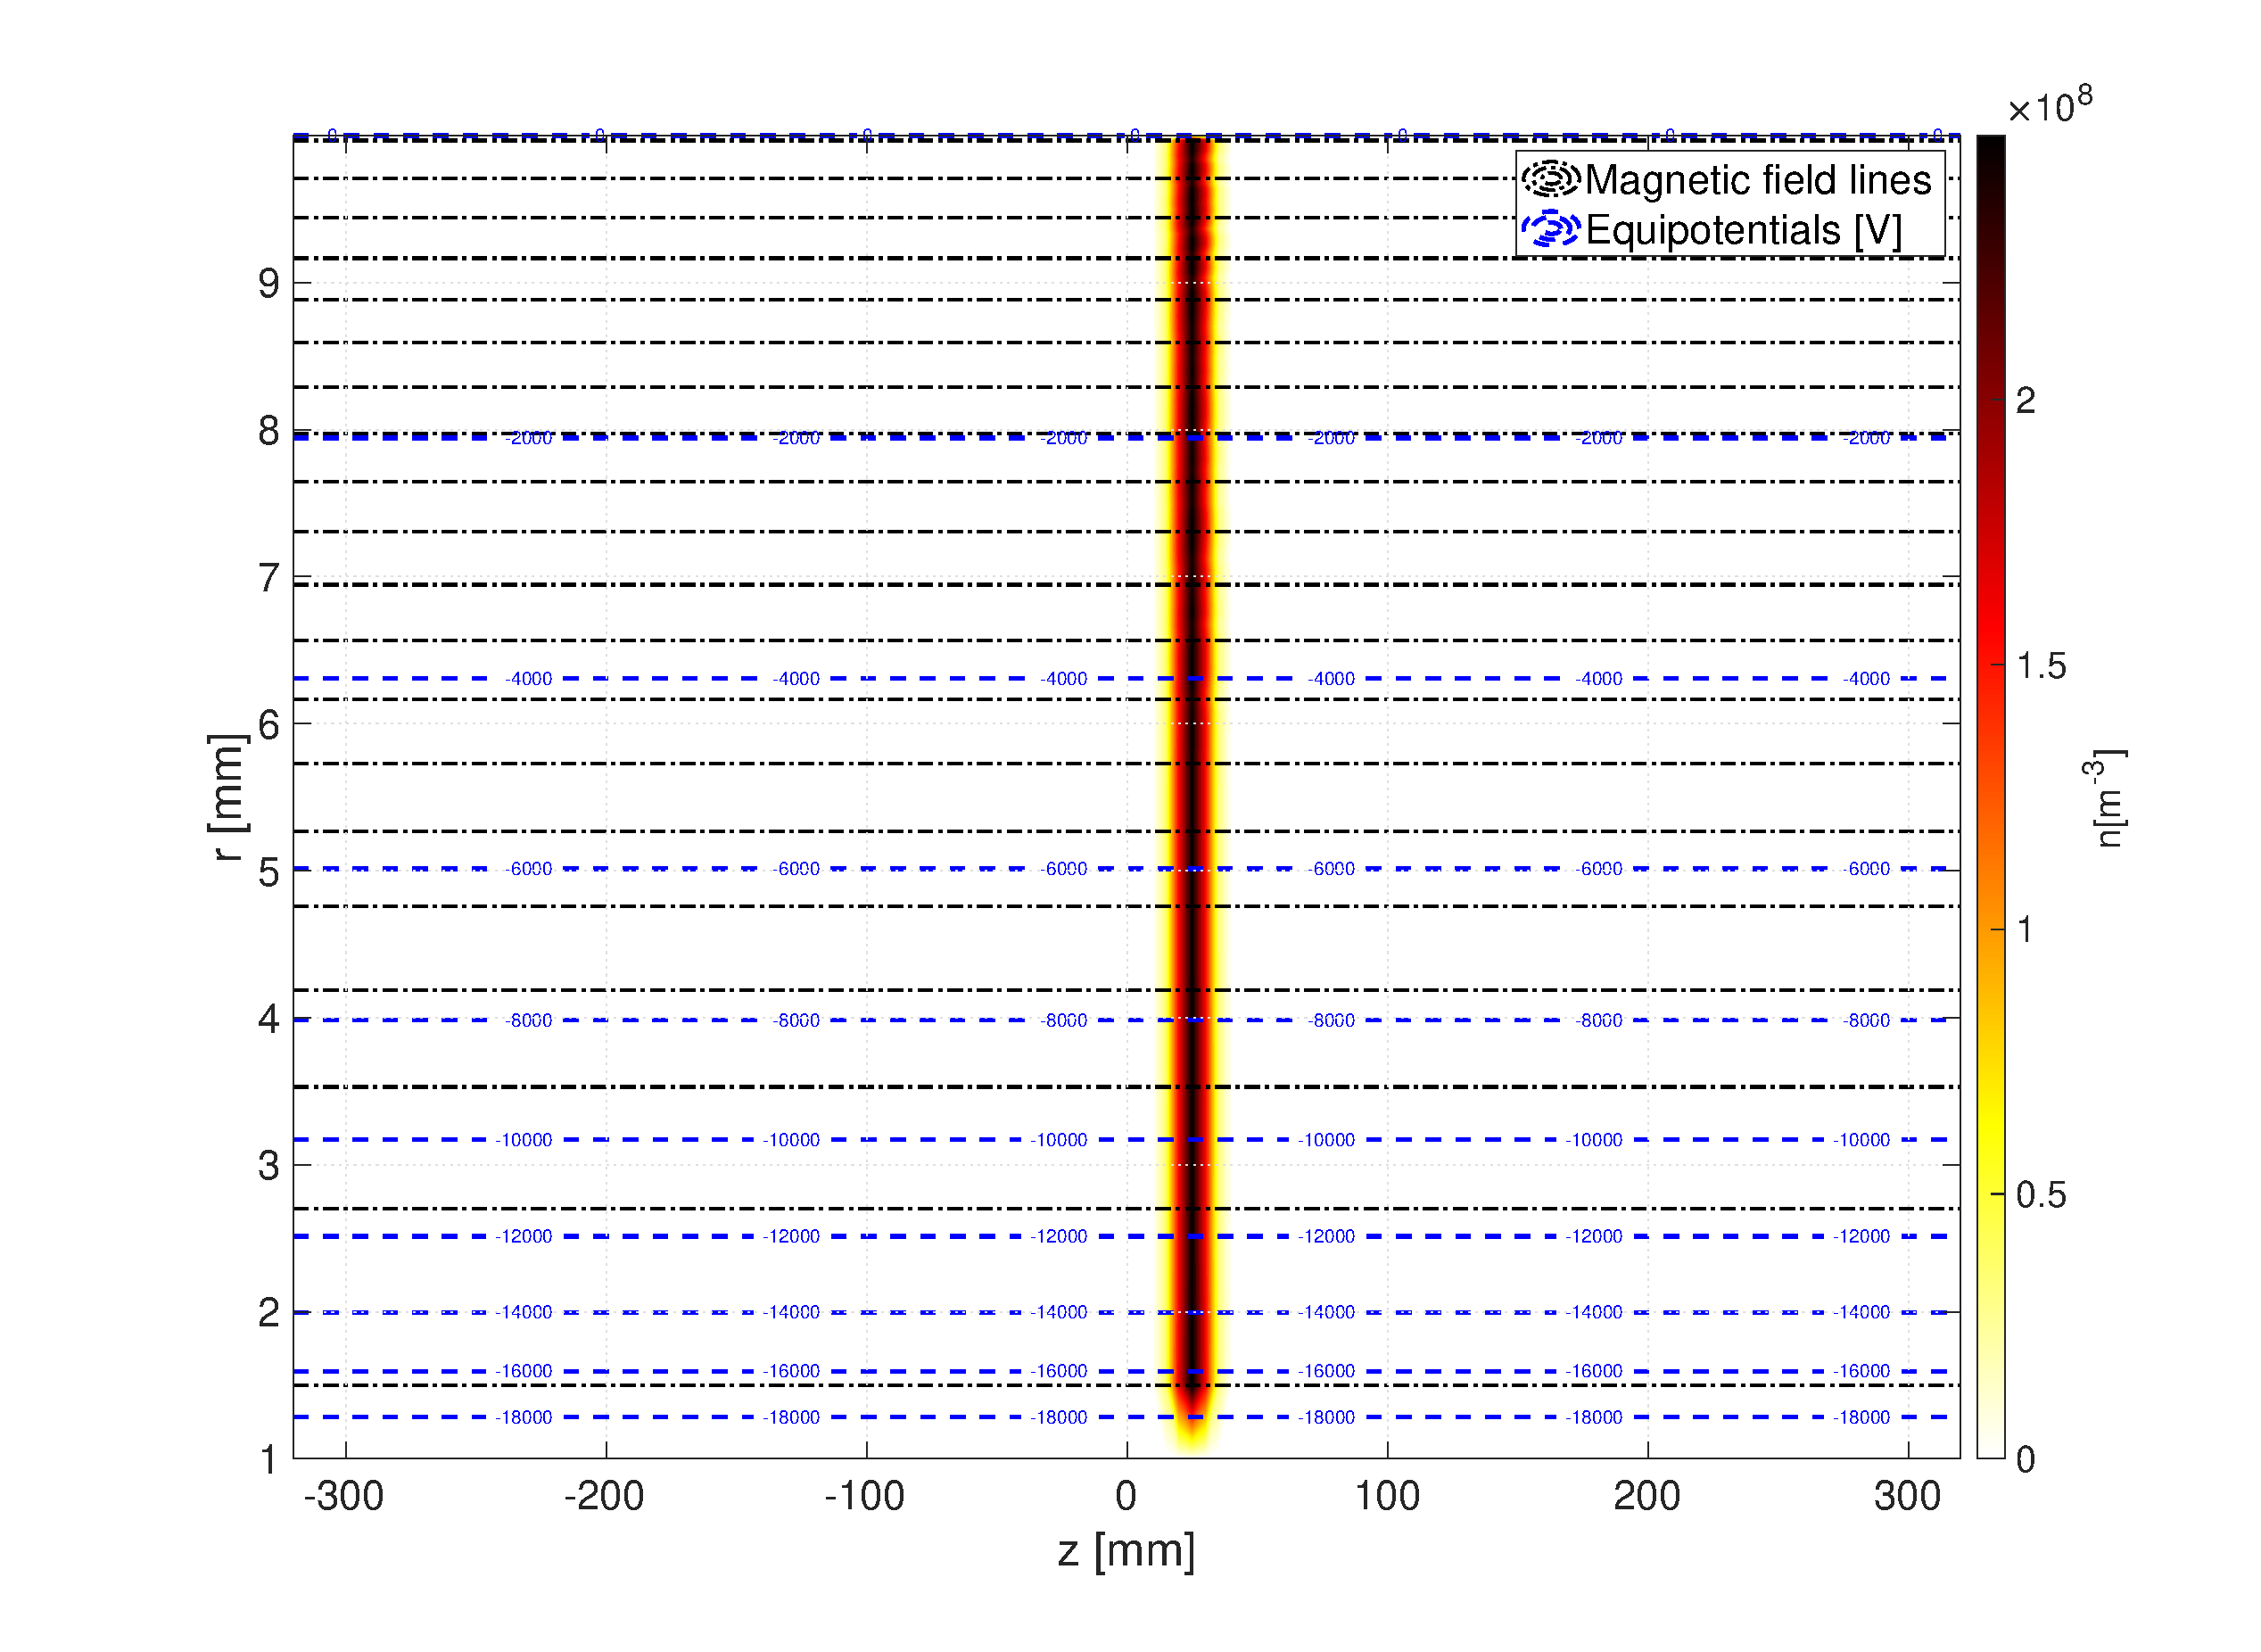
\includegraphics[width=1 \textwidth]{Configuration.eps}
		\caption{\label{config} Initial ion density profile}
		\end{figure}
     \end{columns}
\end{frame}


% %------------------------------------------------
%%%%%%%%%%%%%%%%%%%%



\begin{frame}{Energy collected at the electrode}
     \begin{columns}[c] % The "c" option specifies centered vertical alignment while the "t" option is used for top vertical alignment

         \column{.5\textwidth} % Left column and width
		\begin{figure}[h!]
		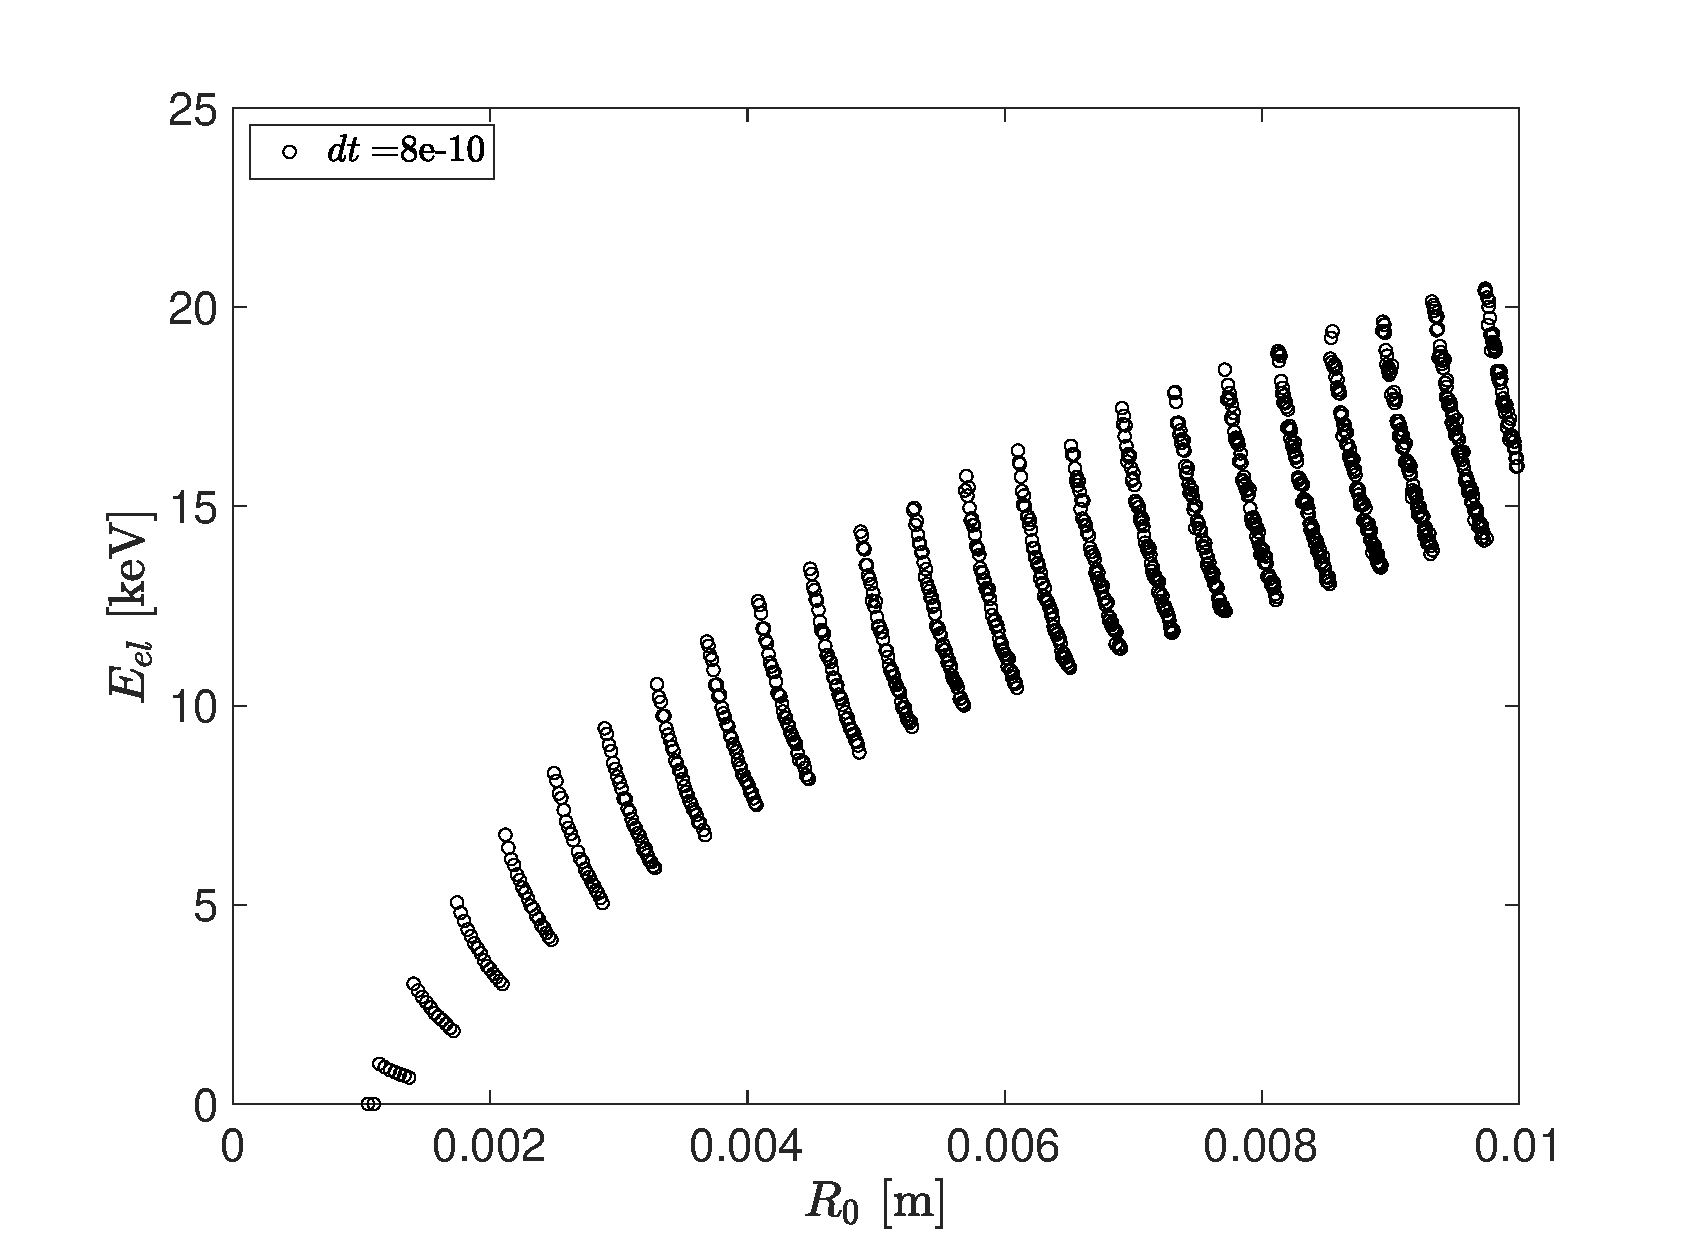
\includegraphics[width=1 \textwidth]{E(R0)_9.eps}
		\caption{\label{config} Energy collected at the electrode - $dt = 8e^{-10}$}
		\end{figure}

         \column{.5\textwidth} % Right column and width
		\begin{figure}[h!]
		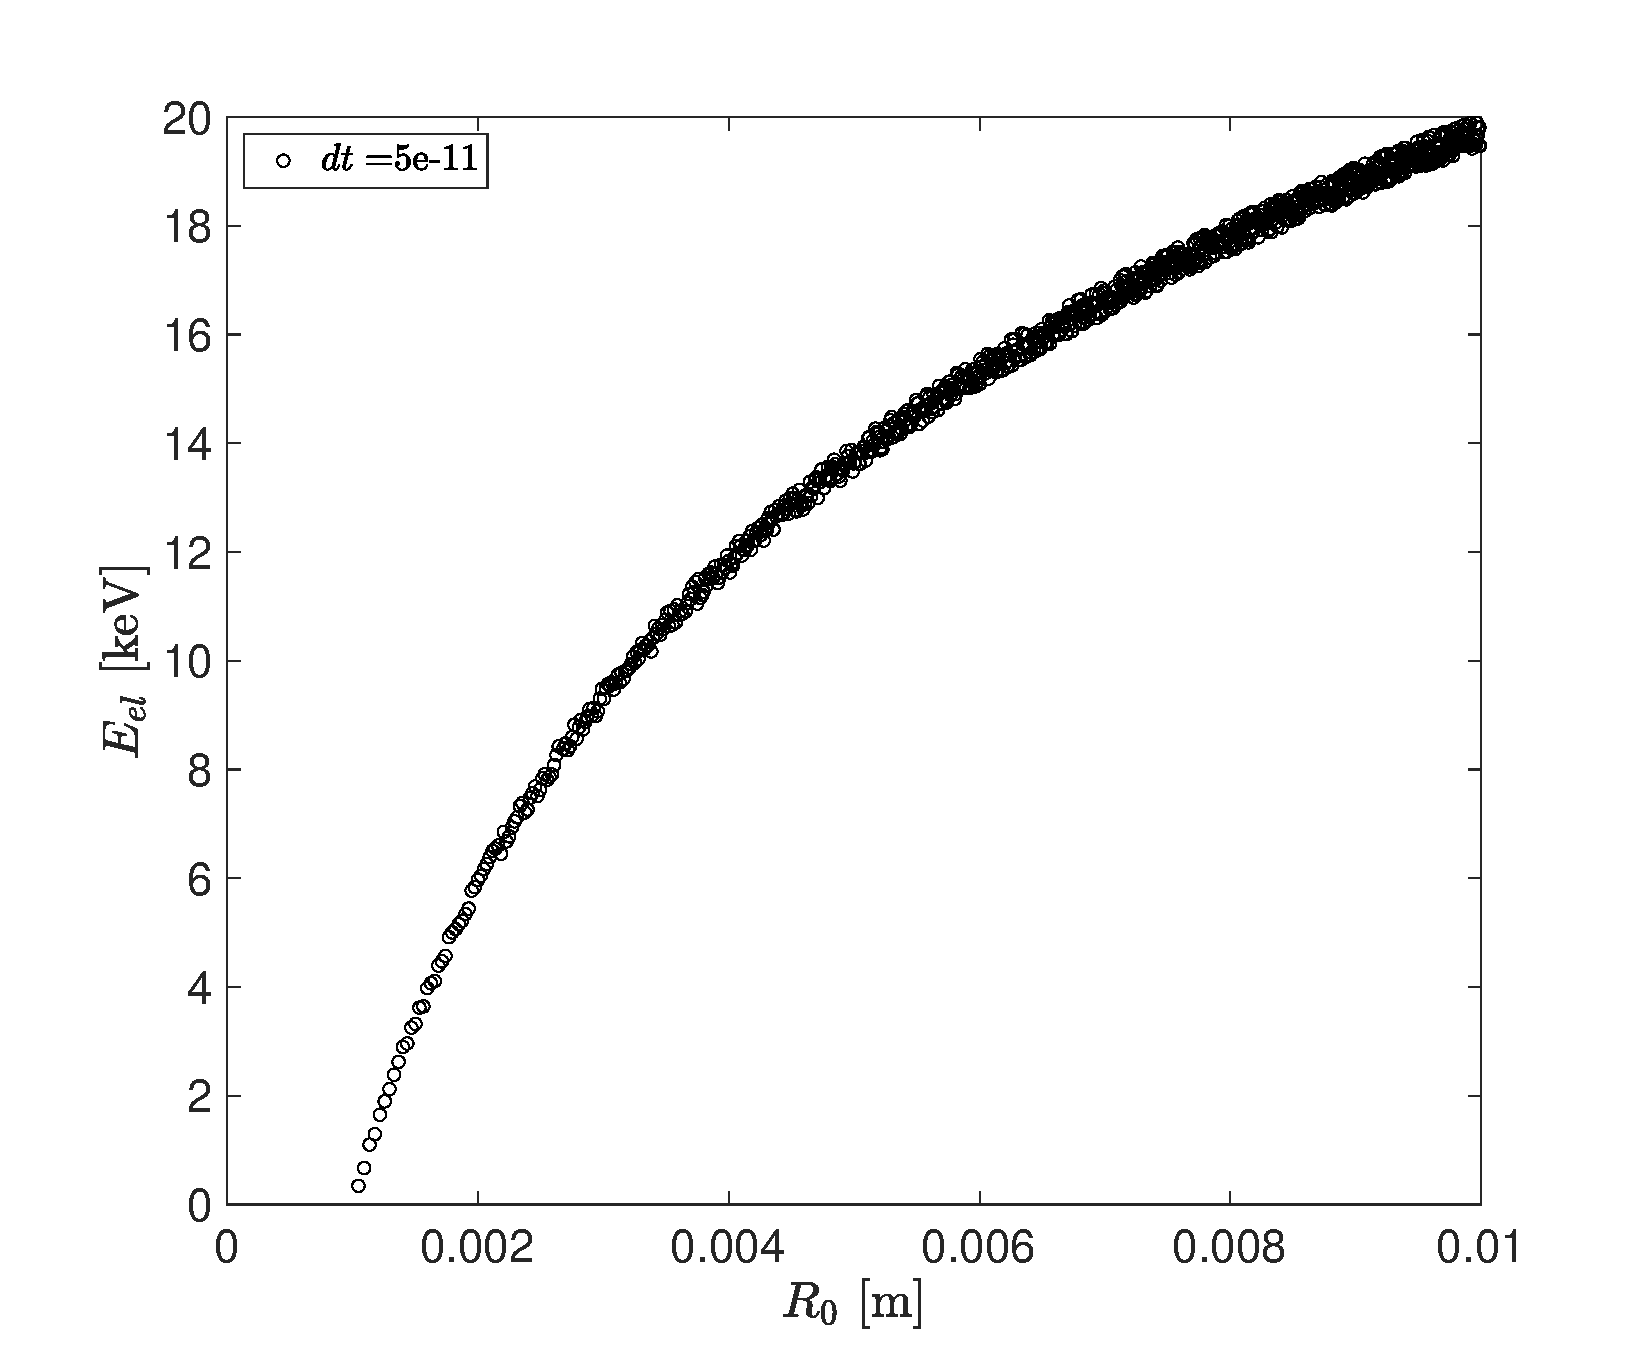
\includegraphics[width=1 \textwidth]{E(R0)_11.eps}
		\caption{\label{config} Energy collected at the electrode - $dt = 1e^{-11}$}
		\end{figure}
     \end{columns}
\end{frame}

%%%%%%%%%%%%%%%%%%%%%%%%%%%%%%%%%%


\begin{frame}{Kinetic energy and energy loss $dE/dx$}
     \begin{columns}[c] % The "c" option specifies centered vertical alignment while the "t" option is used for top vertical alignment

         \column{.5\textwidth} % Left column and width
		\begin{figure}[h!]
		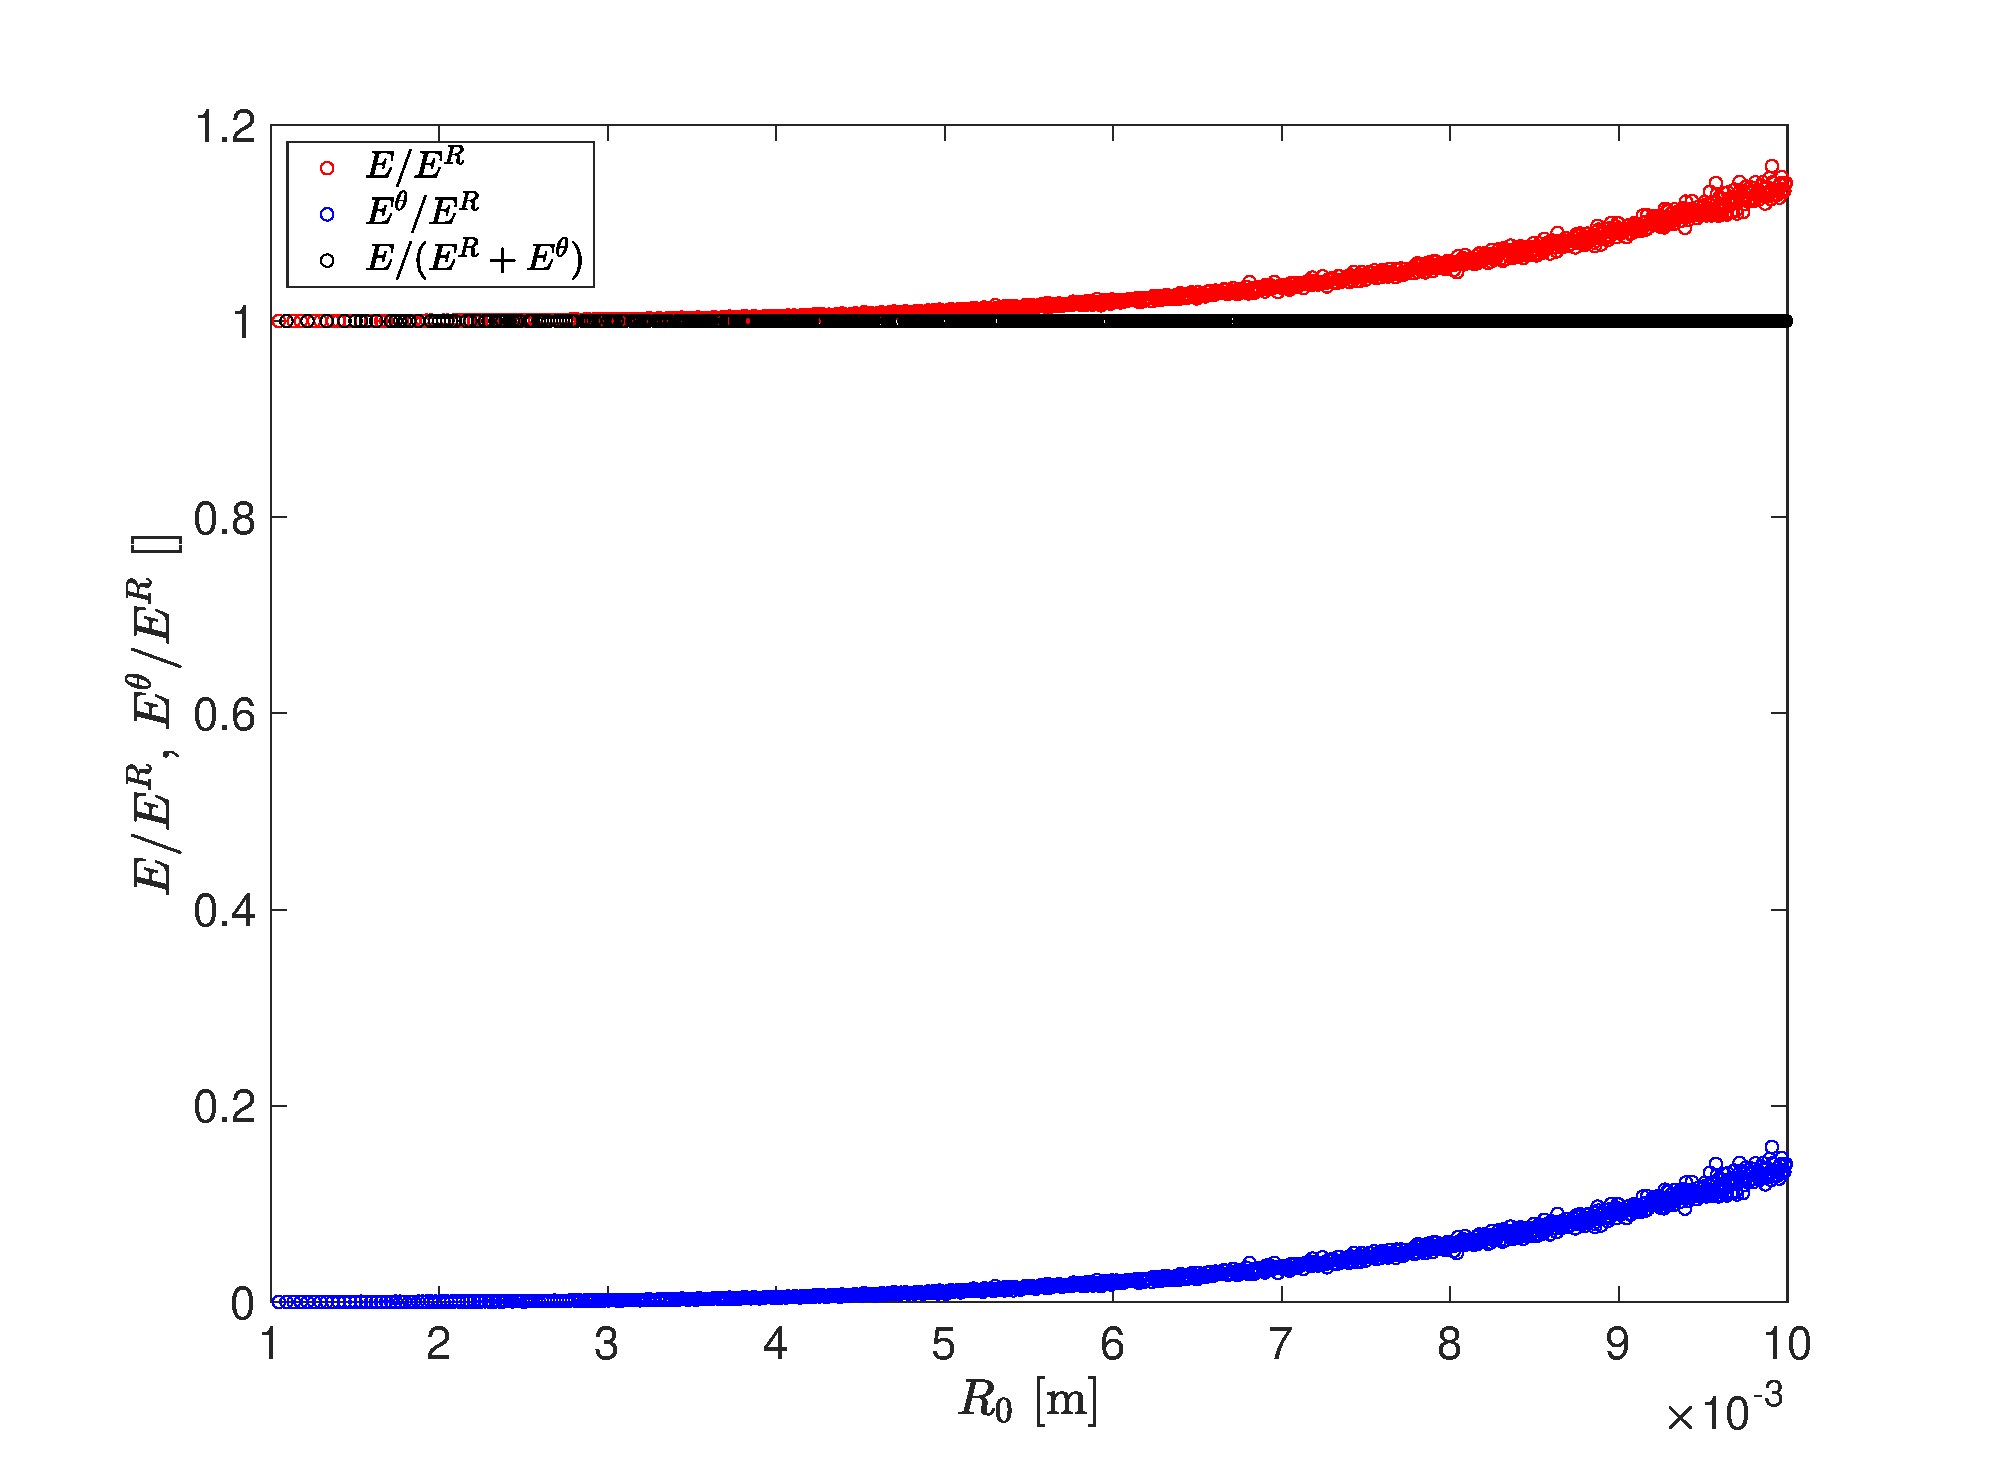
\includegraphics[width=1.1 \textwidth]{ER_11.eps}
		\caption{\label{config} Ratio of the different components of kinetic energy}
		\end{figure}

         \column{.5\textwidth} % Right column and width
		\begin{figure}[h!]
		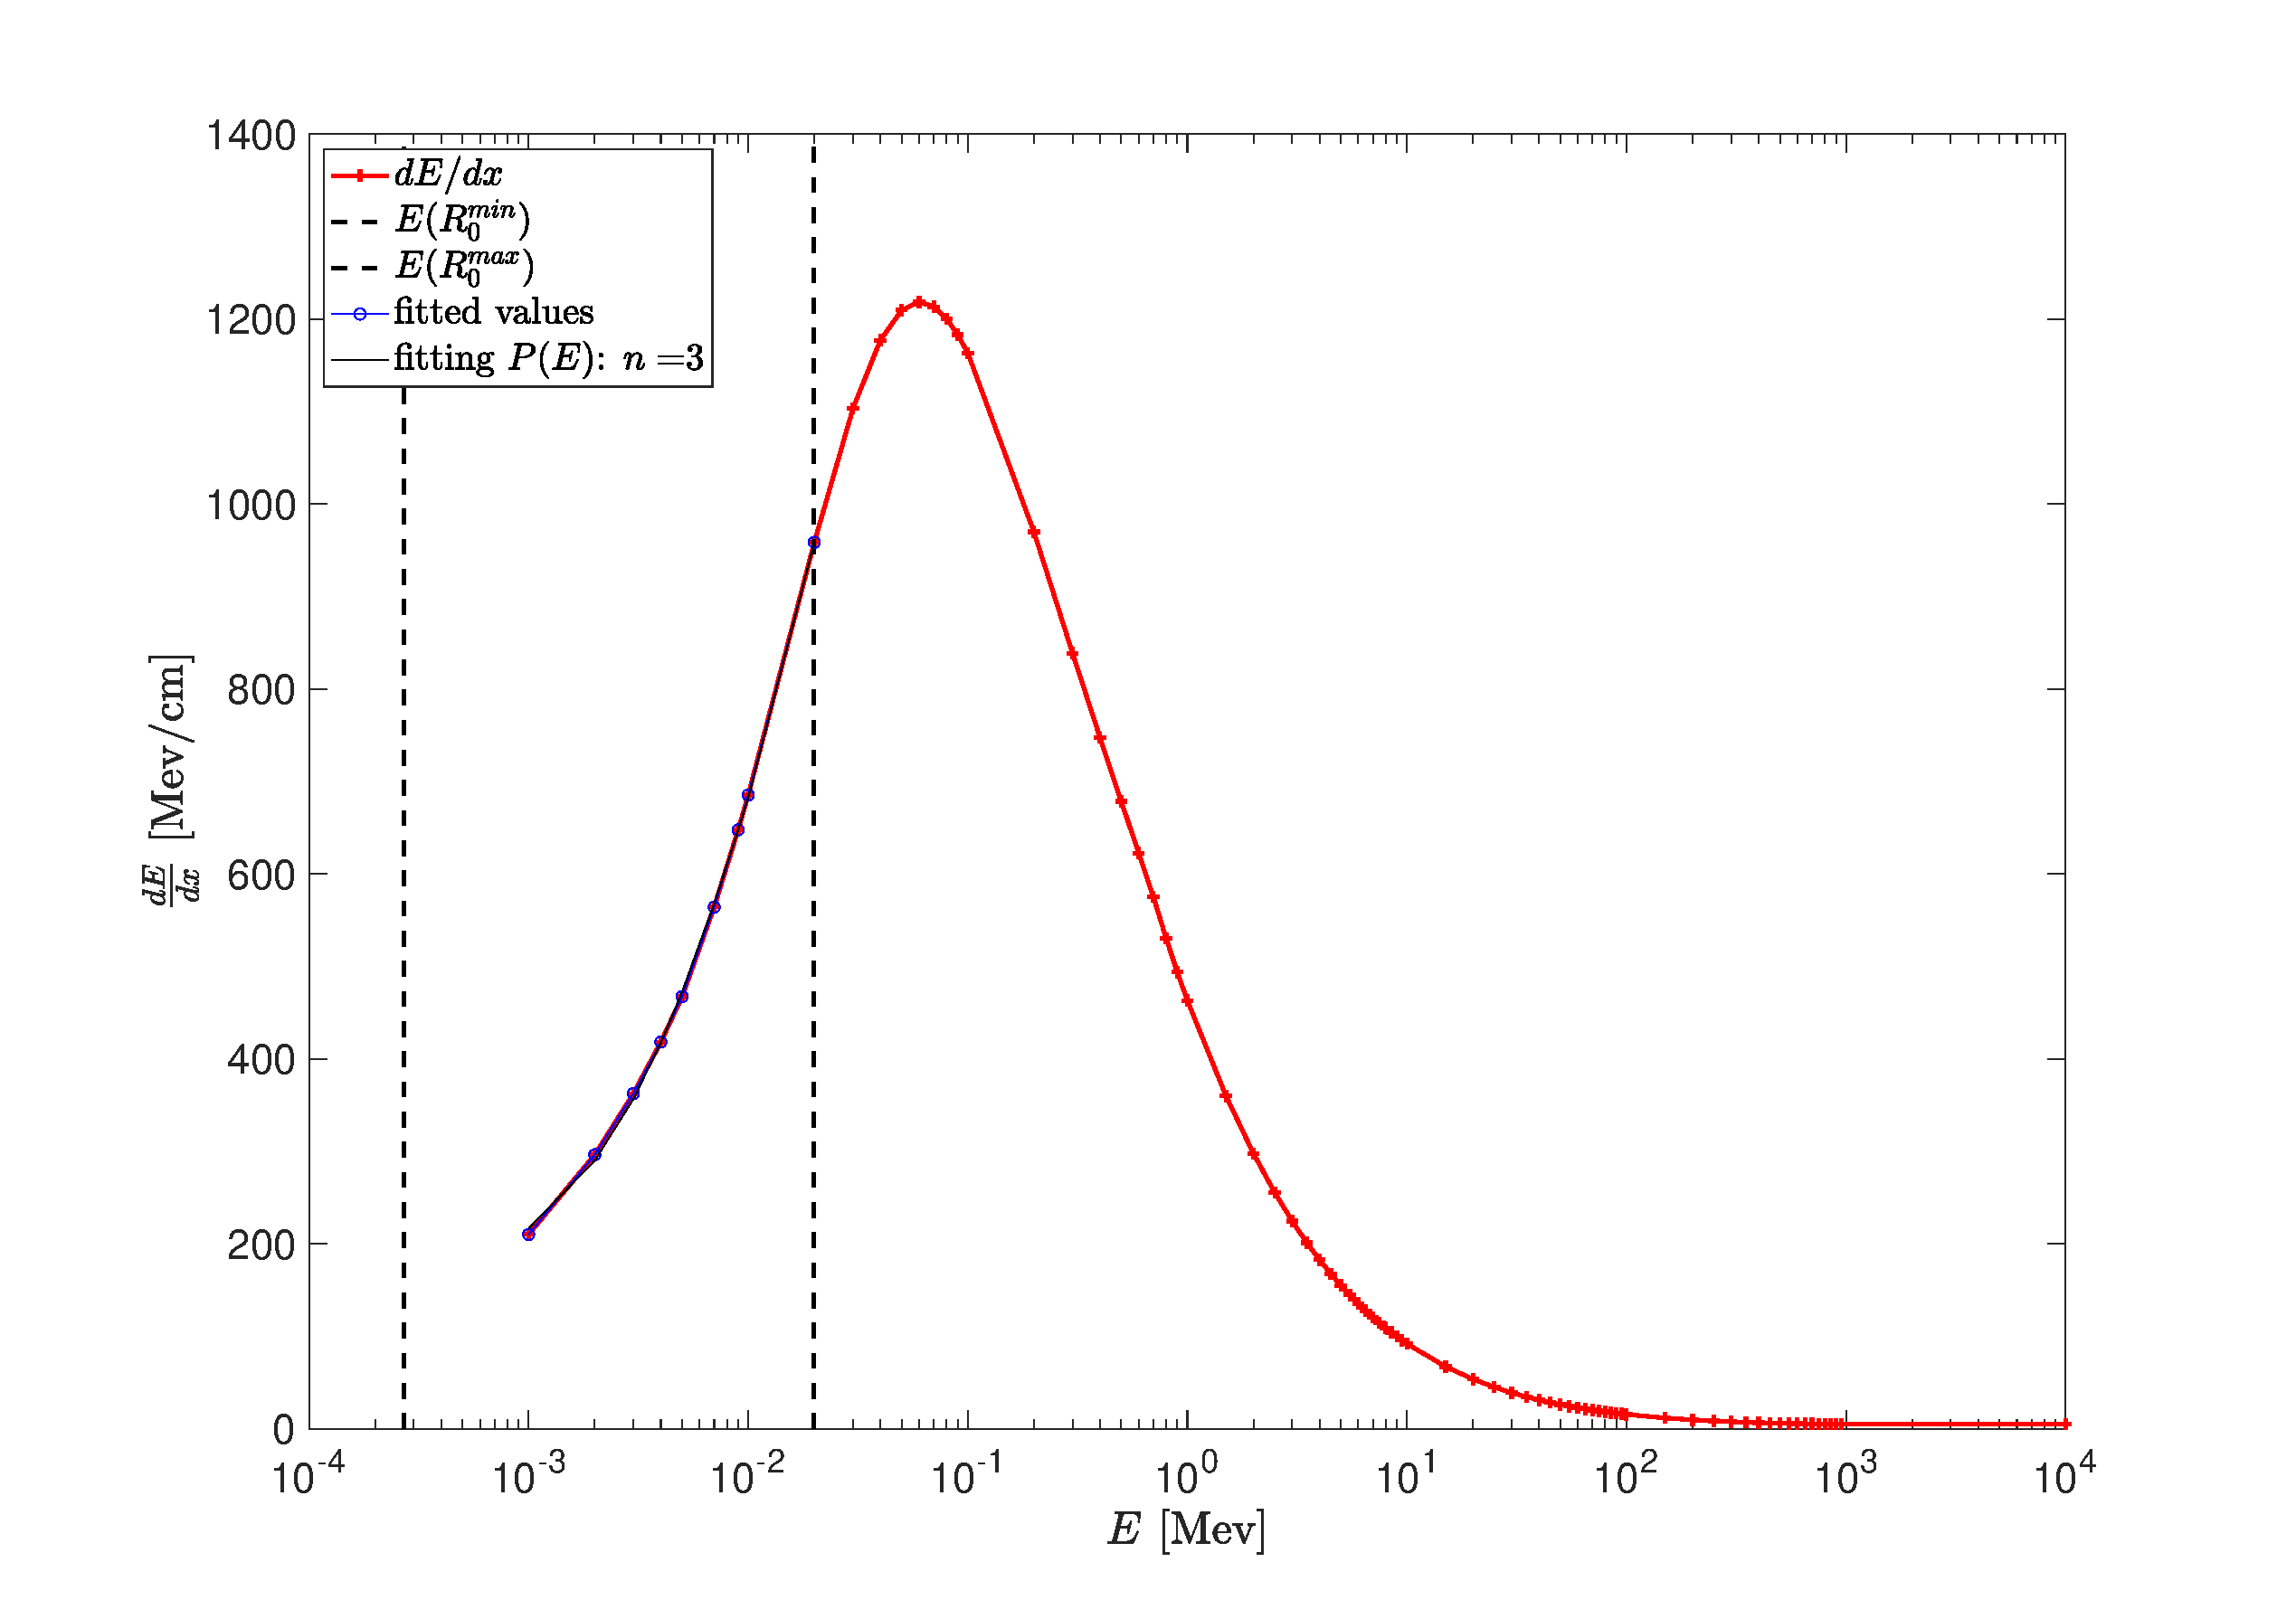
\includegraphics[width=1.1 \textwidth]{ElossFit3AllPts.eps}
		\caption{\label{config}Energy loss and energy range of interest with polynomial fit}
		\end{figure}
     \end{columns}
\end{frame}

%%%%%%%%%%%%%%%%%%%%%%%%%%%%

\begin{frame}{Electron yield - Kinetic theory}
		\begin{figure}[h!]
		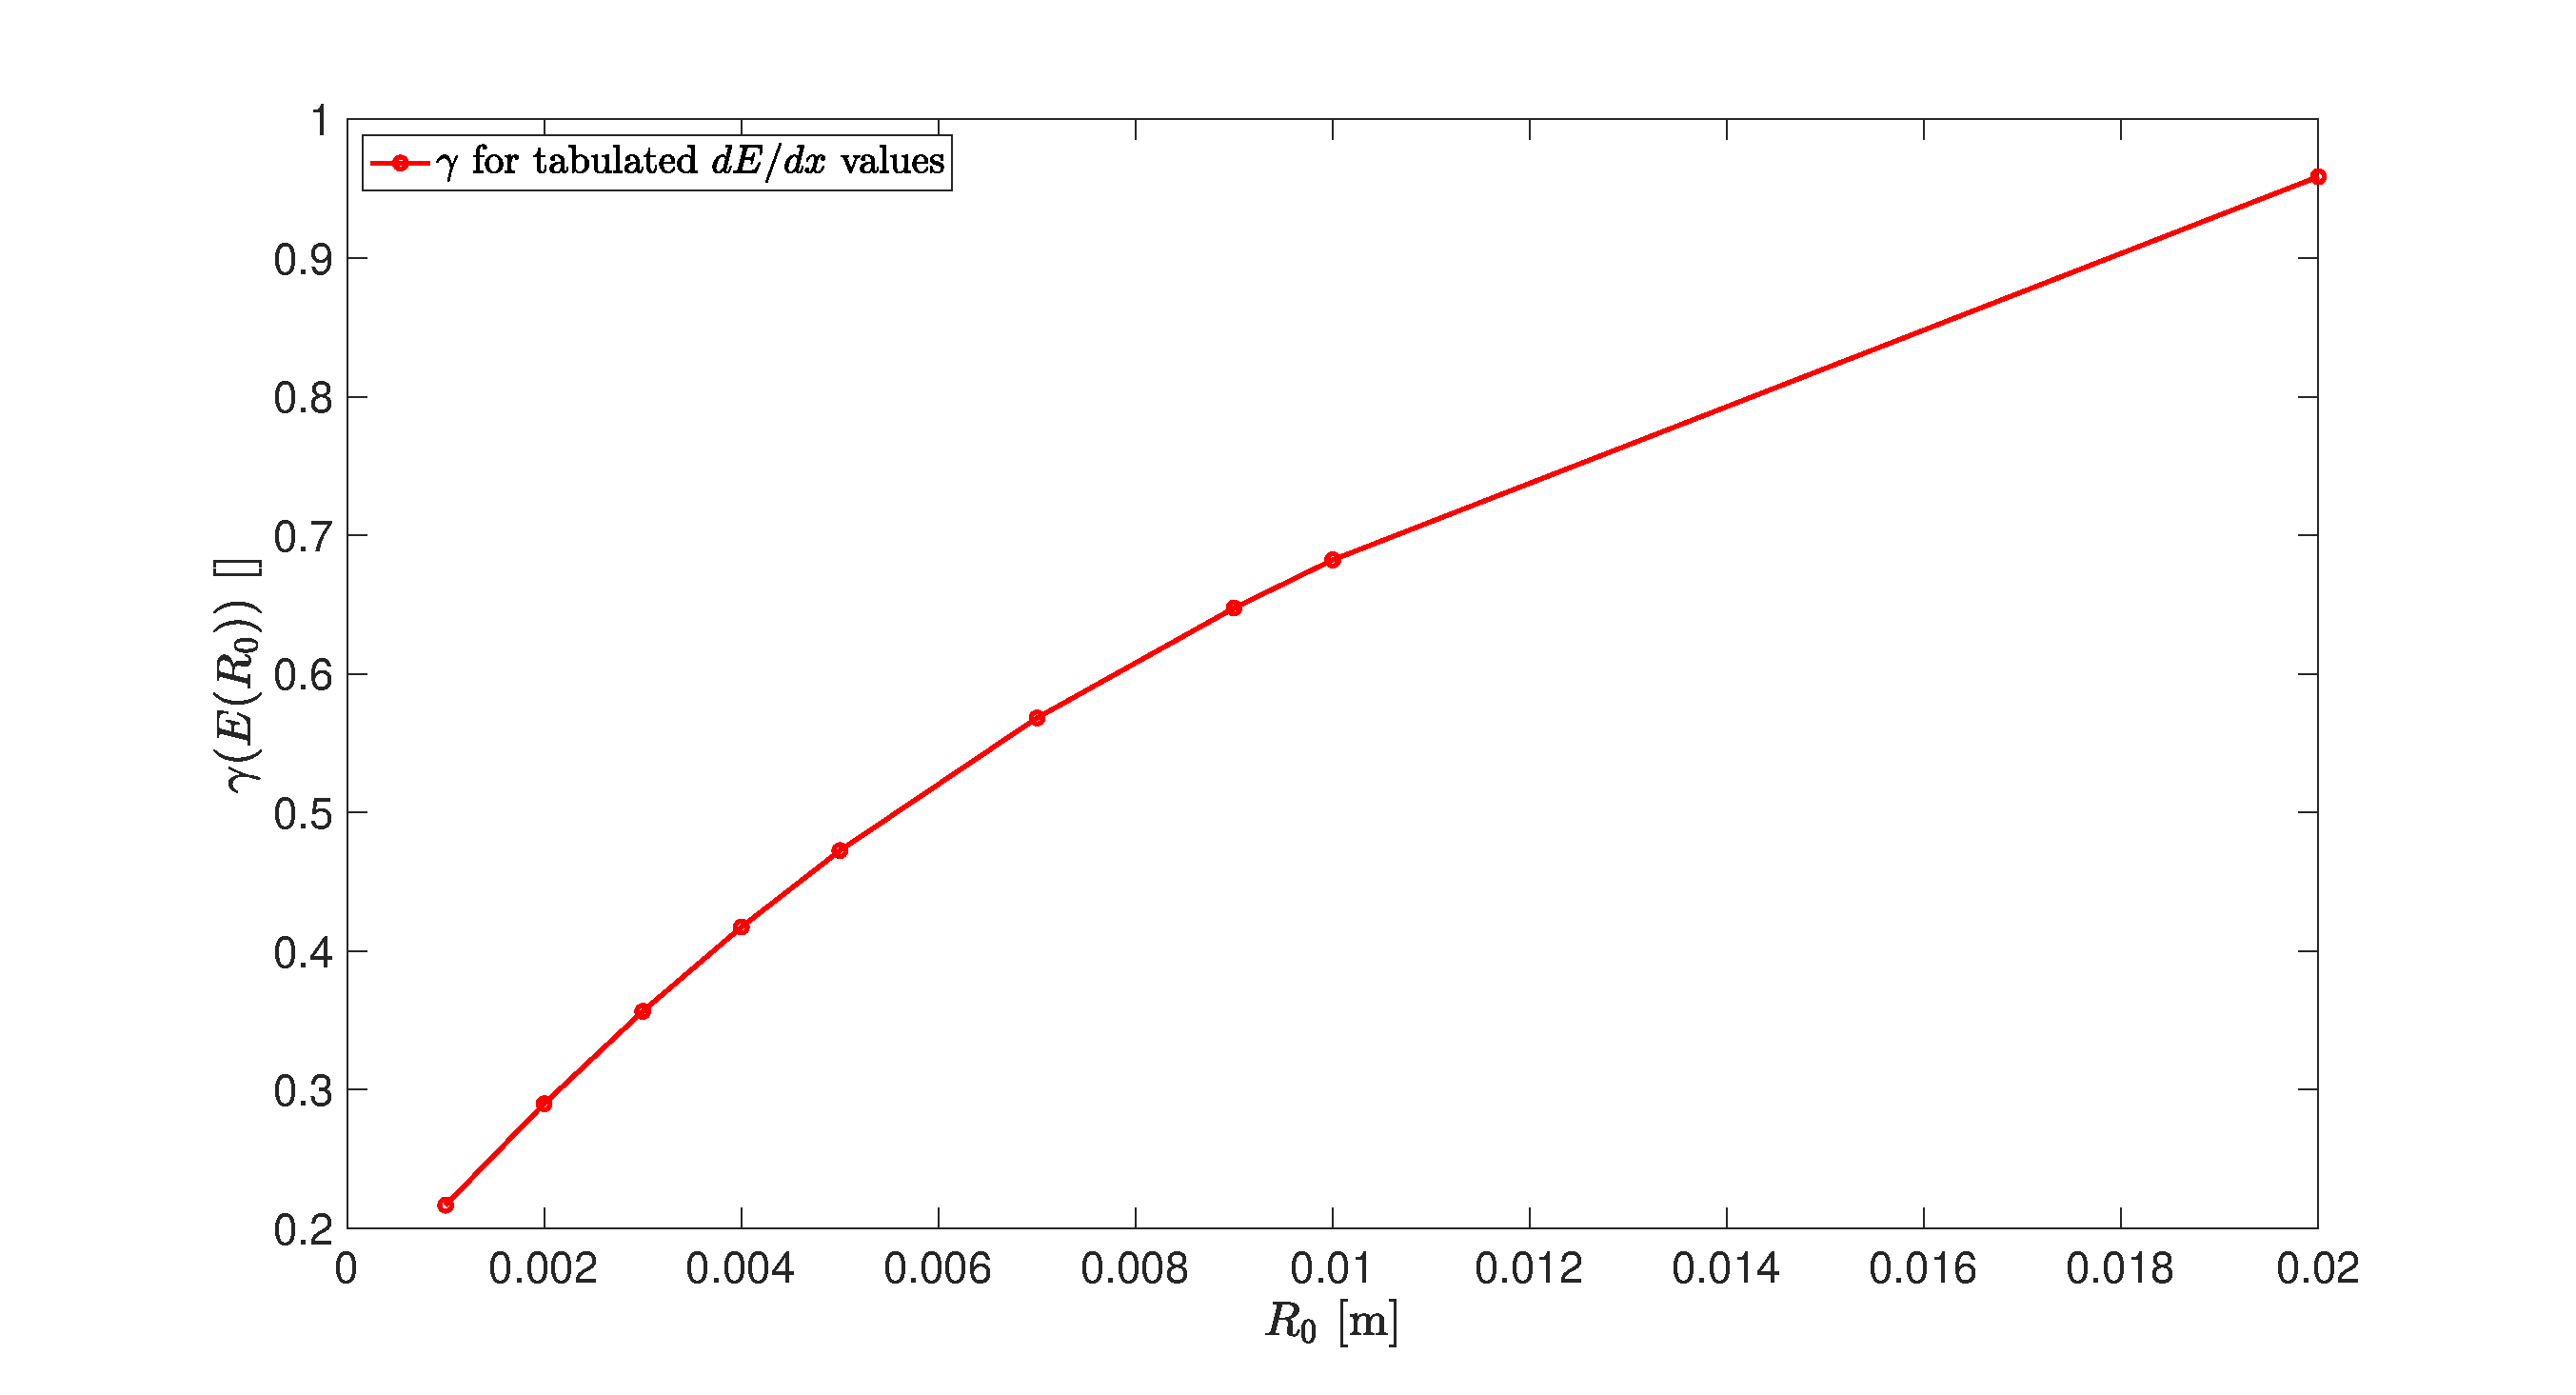
\includegraphics[width=1 \textwidth]{YieldFit3AllPts.eps}
		\caption{\label{config}Yield over the fitted energy interval, given as a function of the energy through $R_0$}
		\end{figure}
\end{frame}






% %------------------------------------------------
%%%%%%%%%%%%%%%%%%%%

\end{document}

